\begin{solution}{normal}
According to Prevost’s theory of exchange, in order to maintain thermal equilibrium, any object must
emit the same energy as it receives. The power recieved is $IA_{\text{eff}}$ and the power emmited is $\sigma 6s^2 T^4$, where $s$ is the sidelength of the cube. This then tells us that 
\[IA_{\text{eff}} = \sigma 6s^2 T^4\implies T = \sqrt[4]{\frac{IA_{\text{eff}}}{\sigma 6s^2}}.\]
We now have to analyze the extremas of $A_{\text{eff}}$.
\begin{enumerate}
    \item $A_{\text{eff}}$ is minimum when the cube recieves the beam directly on the center of its face. This means that $A_{\text{min}} = s^2\implies T = \sqrt{\dfrac{I}{6\sigma}}$.
    \item The maximum is achieved when two space opposite vertices are aligned with the direction of the beam. This would then mean that the projection is a regular hexagon as shown below. 
    \begin{center}
    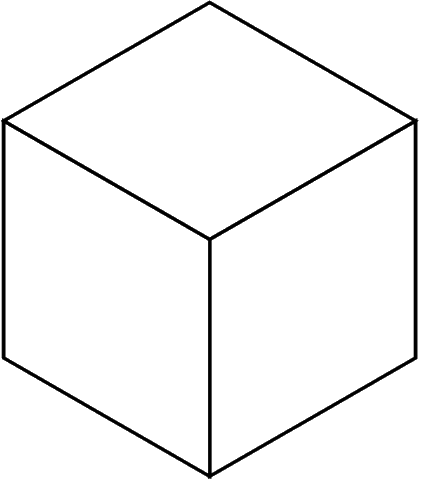
\includegraphics[width=6cm]{Hexagon_in_cube.svg.png}
    \end{center}
    However, the side length of this hexagon is not $s$ because the edges are not parallel to the projection plane. However, if you take the three vertices of the hexagon closest to you and connect these points to make an equilateral triangle, the sides of this triangle will be parallel to the projection plane. The sides of the equilateral triangle are face diagonals and have length $s\sqrt{2}$. The area of the hexagon is twice the area of the equilateral triangle and therefore has area $\frac{\sqrt{3}}{2}(s\sqrt{2})^2=s^2\sqrt{3}$. Therefore $T_{\text{max}}=\sqrt[4]{\dfrac{I\sqrt{3}}{\sigma 6}}$
\end{enumerate}
\blfootnote{Credits to \url{https://commons.wikimedia.org/wiki/File:Hexagon_in_cube.svg} for the image source.}
\tcbline
\textbf{Solution 2.} 
Once again, according to Prevost’s theory of exchange, in order to maintain thermal equilibrium, any object must emit the same energy as it receives. Let the power recieved be $\alpha IA$ and the power emmited is $\sigma 6s^2 T^4$. We then have that 
\[\alpha IA = \sigma 6s^2 T^4\implies T = \sqrt[4]{\frac{\alpha I}{6\sigma}}.\]
The projection of area $A = A \vec n \cdot \vec i $ where $\vec i$ is unit vector in direction of incoming flux, and $\vec n$ is unit vector in direction perpendicular to plane containing the mentioned area. The projection of area is $A = A \vec n \cdot \vec i $ where $\vec i$ is unit vector in direction of incoming flux, and $\vec n$ is unit vector in direction perpendicular to plane containing the mentioned area. Therefore, we have that $\alpha = \sum \vec n \cdot \vec i$. There can be at most $3$ faces with positive projections of area. Let these $3$ faces be in $x,y,z$ directions. Then $\alpha = (\vec n_x + \vec n_y + \vec n_z)\cdot \vec i$ where $n_x = n_y = n_z = 1$ as these are unit vectors. Let $i= \vec i_x + \vec i_y + \vec i_z)$. Then $\alpha = i_x + i_y + i_z$. Since $i$ is unit vector $i_x^2 +i_y^2 +i_z^2 =1$. Also, $0\leq i_x,i_y,i_z \leq 0$ as $\beta^2\geq 0$ for $\beta \in R$ (Note that $i_x,i_y,i_z$ cannot be all equal to zero). Therefore, $i_x^2 \leq i_x,i_y^2\leq i_y,i_z^2\leq i_z \implies i_x^2 +i_y^2 +i_z^2 \leq i_x + i_y + i_z$. We then have by power mean inequality,
$$\frac {i_x + i_y + i_z}{3} \leq \left(\frac {i_x^2 +i_y^2 +i_z^2}{3}\right)^{1/2}$$
This then means that 
$$i_x^2 +i_y^2 +i_z^2 \leq i_x + i_y + i_z \leq \sqrt{3(i_x^2+i_y^2+i_z^2)} $$
which then tells us 
$$1\leq \alpha \leq \sqrt 3.$$
Therefore,
$$T_{\text{max}} = \sqrt[4] {\frac{\sqrt 3 I}{6\sigma}}\, \text{and}\,T_{\text{min}} = \sqrt[4]{\frac{I}{6\sigma}}$$
\end{solution}